\chapter{Results Discussion}
\label{cha:results_discussion}

In this chapter, we analyze the results of our experiments, focusing on how the
agent performs in different maps and goals configuration to evaluate the agent's
ability to navigate the map and successfully complete its tasks. We examine how the
placement of goal tiles affects decision-making, assess whether the model
struggles with retrieving relevant information, and compare the performance in the
same slice of different maps.

Our primary objective is to evaluate the agent's ability to navigate the map and
successfully complete pickup and delivery tasks.

In tasks where the agent's goal is to pick up a parcel, the target tile
corresponds to the one containing the parcel. Conversely, in delivery tasks, the
goal tile is the specific location where the agent must deliver the parcel.

The placement of goal tiles within the game map was carefully designed to ensure
consistency and meaningful evaluation across both pickup and delivery tasks.
Specifically, we aimed to use the same goal tiles for both objectives, allowing
for direct comparisons between the two. In the pickup scenario, the goal is
always explicitly stated at the end of the prompt, making it immediately available
to the LLM. However, in the delivery scenario, the agent must retrieve the
delivery location from the provided map description, requiring it to process and
extract the relevant information effectively.

To evaluate how well the model handles goal retrieval, we selected three
distinct goal positions: the top-right, center, and bottom-right cells of the map.
These placements ensure that the goal appears in different parts of the map
description inside the prompt, allowing us to assess whether the ``needle in a haystack"
problem, as discussed in related literature, affects the model's ability to
locate and act on relevant information during the delivery task.

In the final section, we will discuss the different LLMs used in the agent's decision-making
process. As a general observation, GPT-3.5 performed worse compared to the more advanced
GPT-4o variants. Among the newer models, GPT-4o and GPT-4o-mini demonstrated similar
performance, with both outperforming GPT-3.5. Due to budget constraints, the
majority of our analysis was conducted using GPT-4o-mini, as it provides a cost-effective
yet high-quality alternative. However, our qualitative findings can be reasonably
extended to GPT-4o as well, given their comparable performance, and to all models
with similar performance and/or architecture.

\section{Map Orientation}

In this section, we analyze the impact of map orientation on the agent's decision-making
process. Since the prompt did not explicitly reference any specific orientation,
the model had to infer it based solely on the provided map description and its training
data. By examining the model's outputs, we can determine its perceived orientation
of the map and assess whether any biases emerge.

To investigate this, we analyzed the data using two different origin conventions.
The raw data was structured with the $(0,0)$ coordinate in the top-left corner,
but we also transformed the map to simulate a bottom-left origin by adjusting
all coordinates accordingly. We then ran the agent in both configurations—one using
the original top-left origin and another using the simulated bottom-left origin—to
compare how the agent's actions varied under different map orientations.

As illustrated in Figure \ref{fig:orientation}, the heatmaps of the agent's
actions appear nearly identical, except for a 90-degree rotation. The small
differences between the two cases can be attributed to the way the data was
structured in the prompt, which may have influenced the model's text generation.

\begin{figure}[h]
  \centering
  \begin{minipage}[b]{0.45\textwidth}
    \centering
    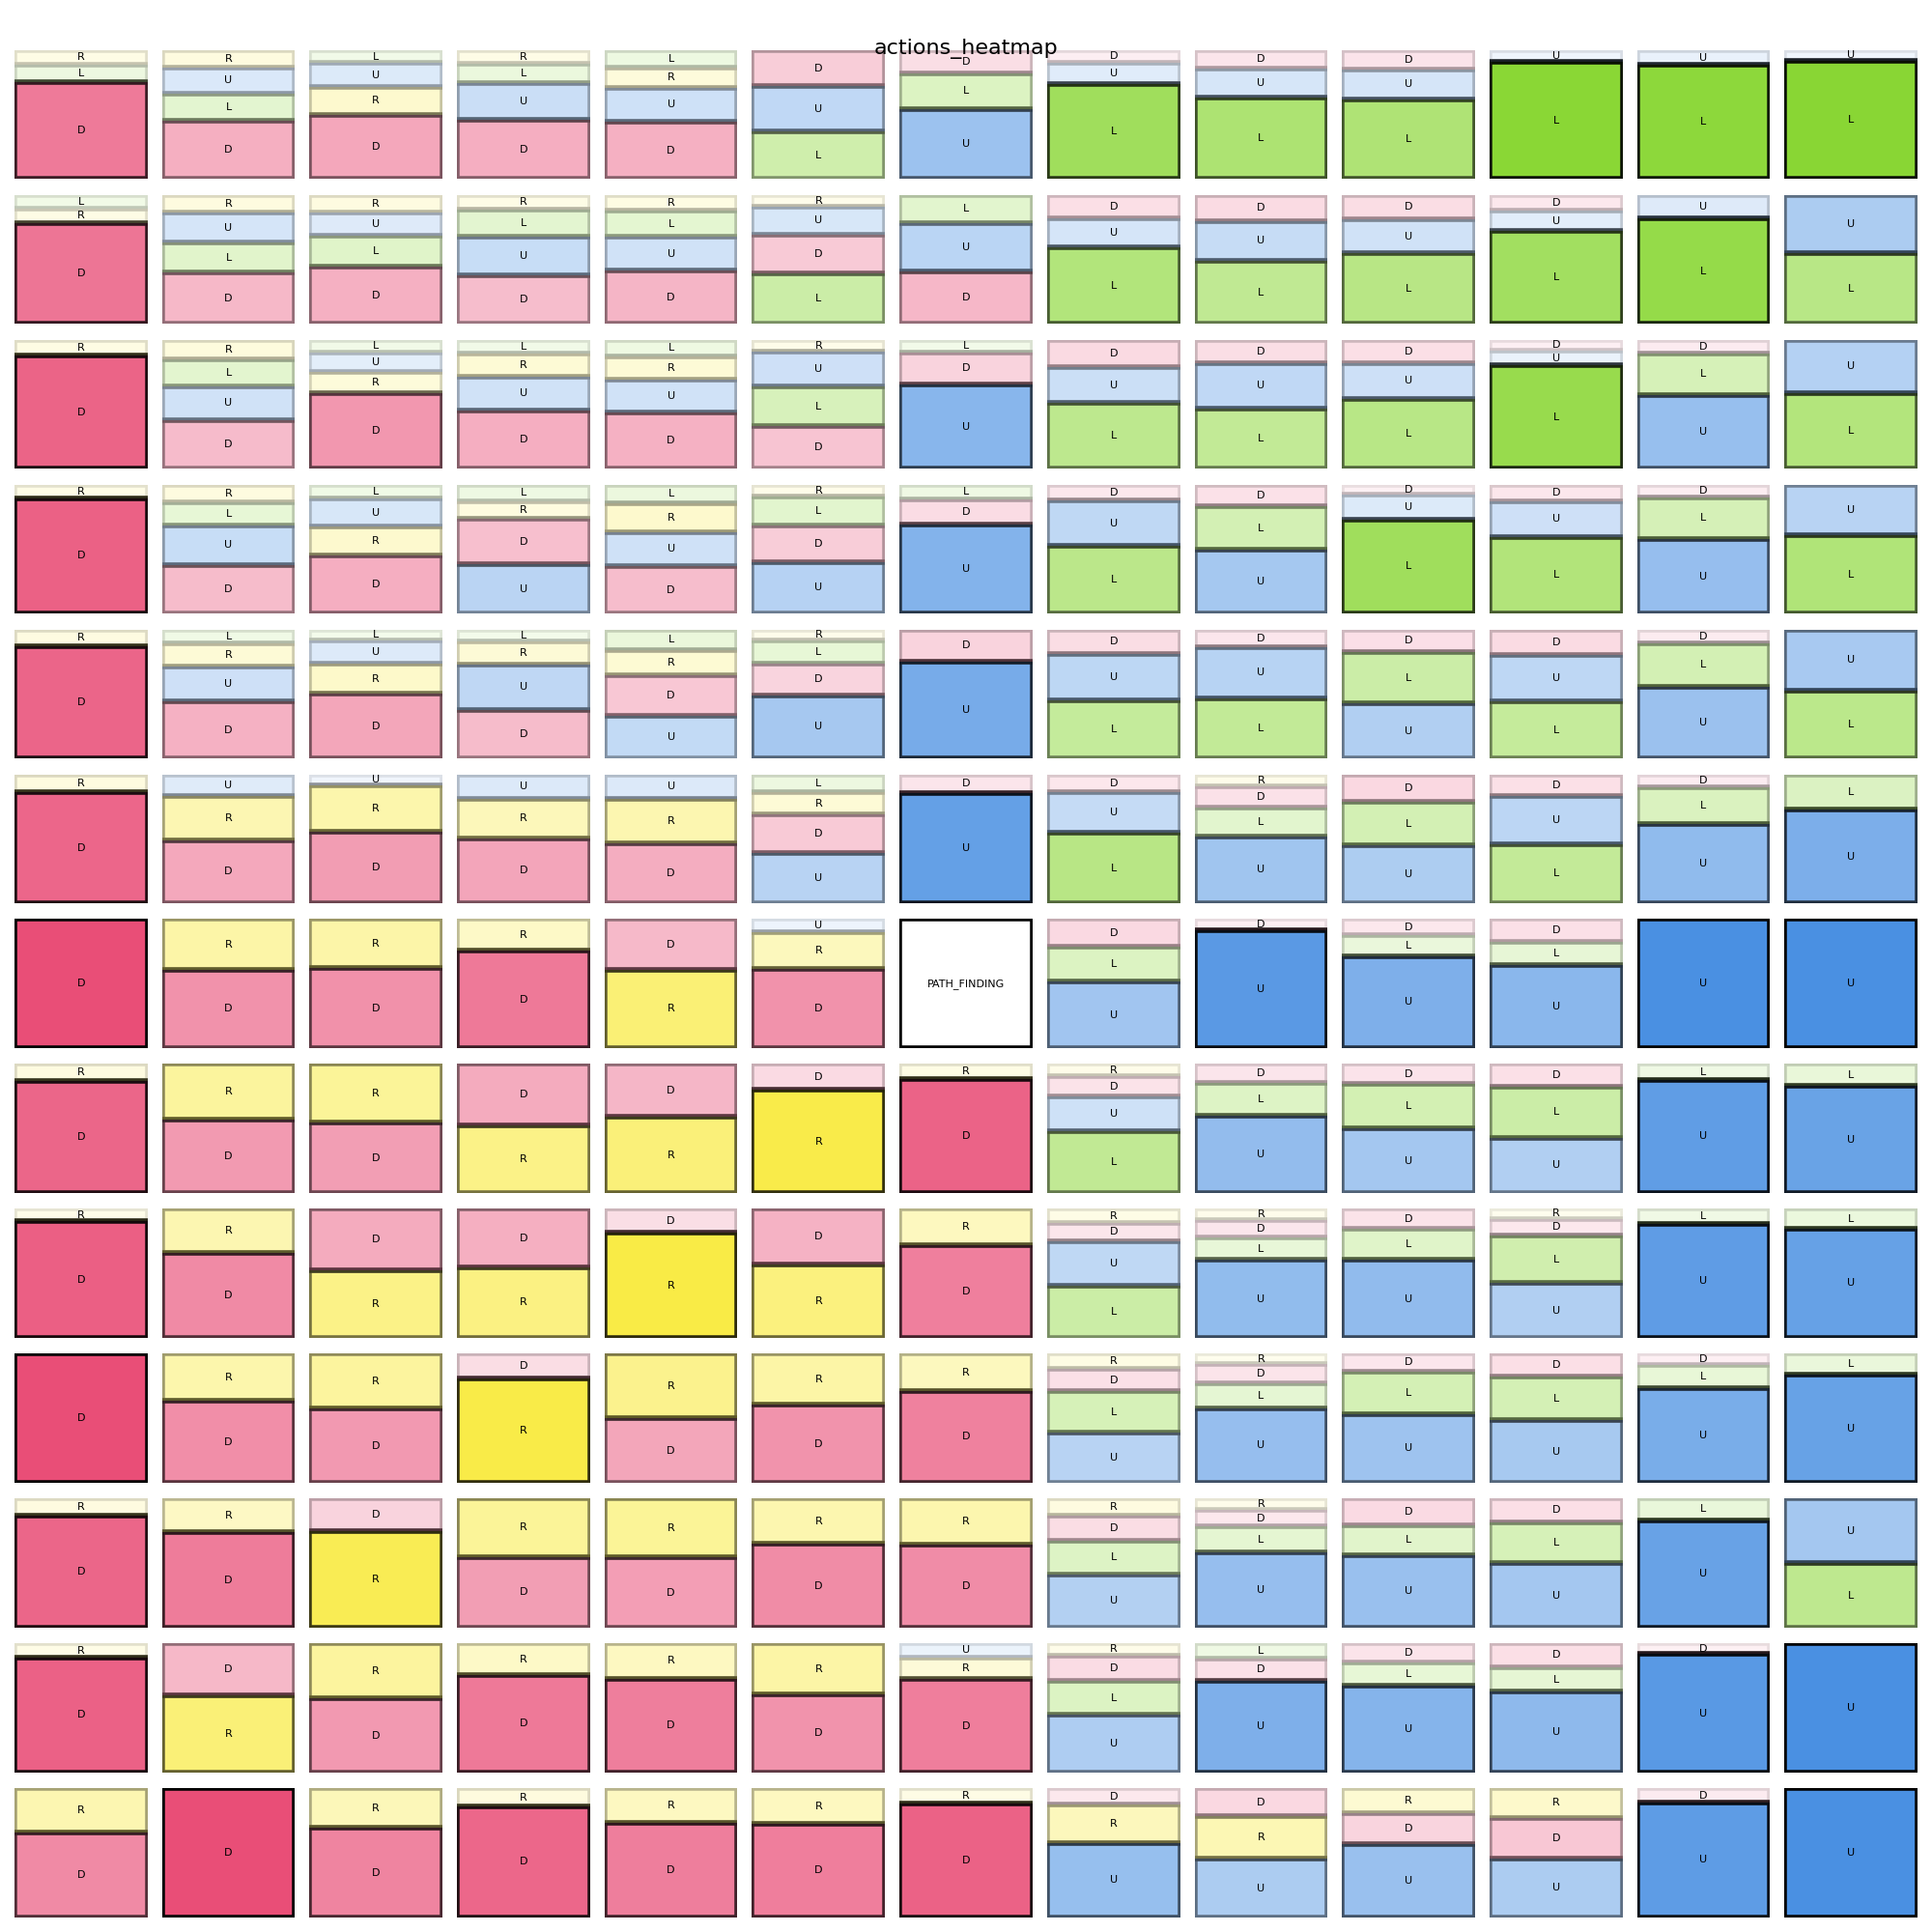
\includegraphics[width=\textwidth]{
      images/results_discussion/actions_heatmapBL.png
    }
    \caption{Bottom Left Orientation}
    \label{fig:heatmapBL}
  \end{minipage}
  \hfill
  \begin{minipage}[b]{0.45\textwidth}
    \centering
    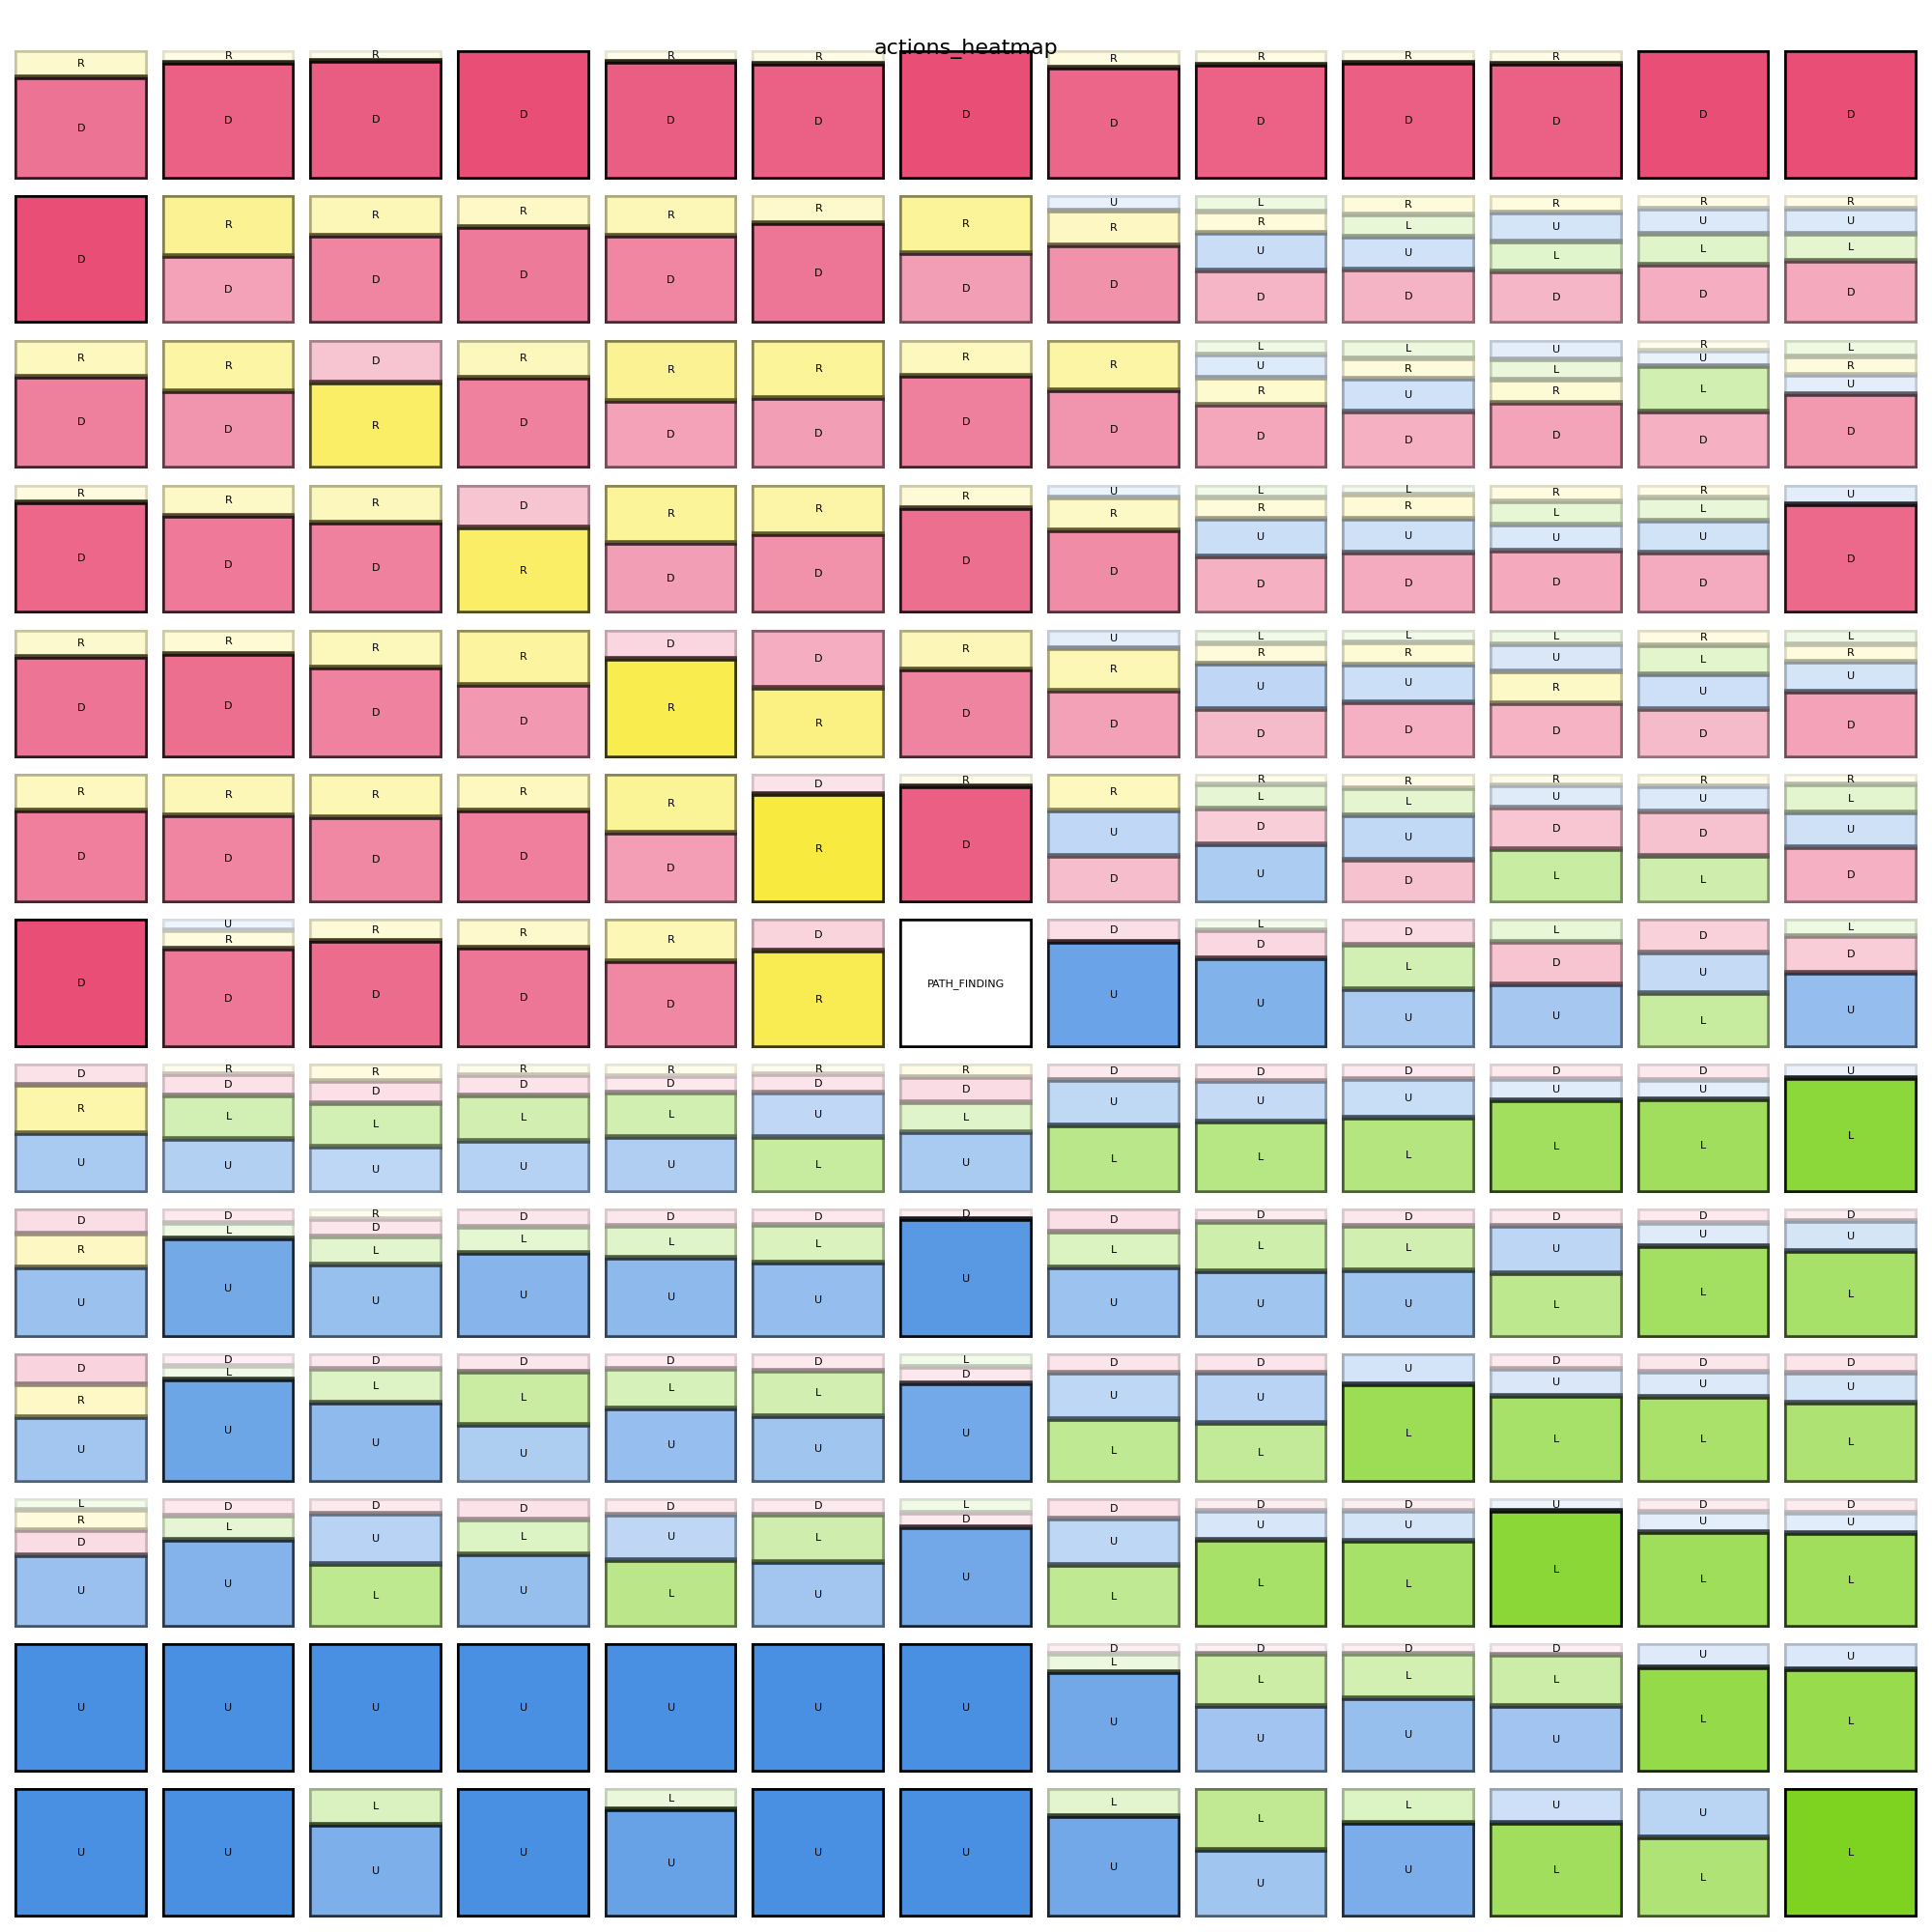
\includegraphics[width=\textwidth]{
      images/results_discussion/actions_heatmapTL.png
    }
    \caption{Top Left Orientation}
    \label{fig:heatmapTL}
  \end{minipage}
  \caption{Heatmaps showing actions with different map orientations}
  \label{fig:orientation}
\end{figure}

To further analyze the effect of orientation, we examined the correctness heatmaps
for both configurations, as shown in Figure \ref{fig:orientation_correctness}. The
results reveal a clear bias toward the top-left origin orientation, which we
refer to as the "programming origin," in contrast to the "Cartesian origin" commonly
used in mathematical contexts.

This bias may stem from the way the map was presented to the model. In our
specific implementation, the map was formatted as a list of tiles extracted from
a minimally edited JSON file. Given that JSON and other common data structures
in computer science often follow a top-left origin convention, it is likely that
the LLM was implicitly influenced by its prior knowledge from programming-related
contexts.

\begin{figure}[h]
  \centering
  \begin{minipage}[b]{0.45\textwidth}
    \centering
    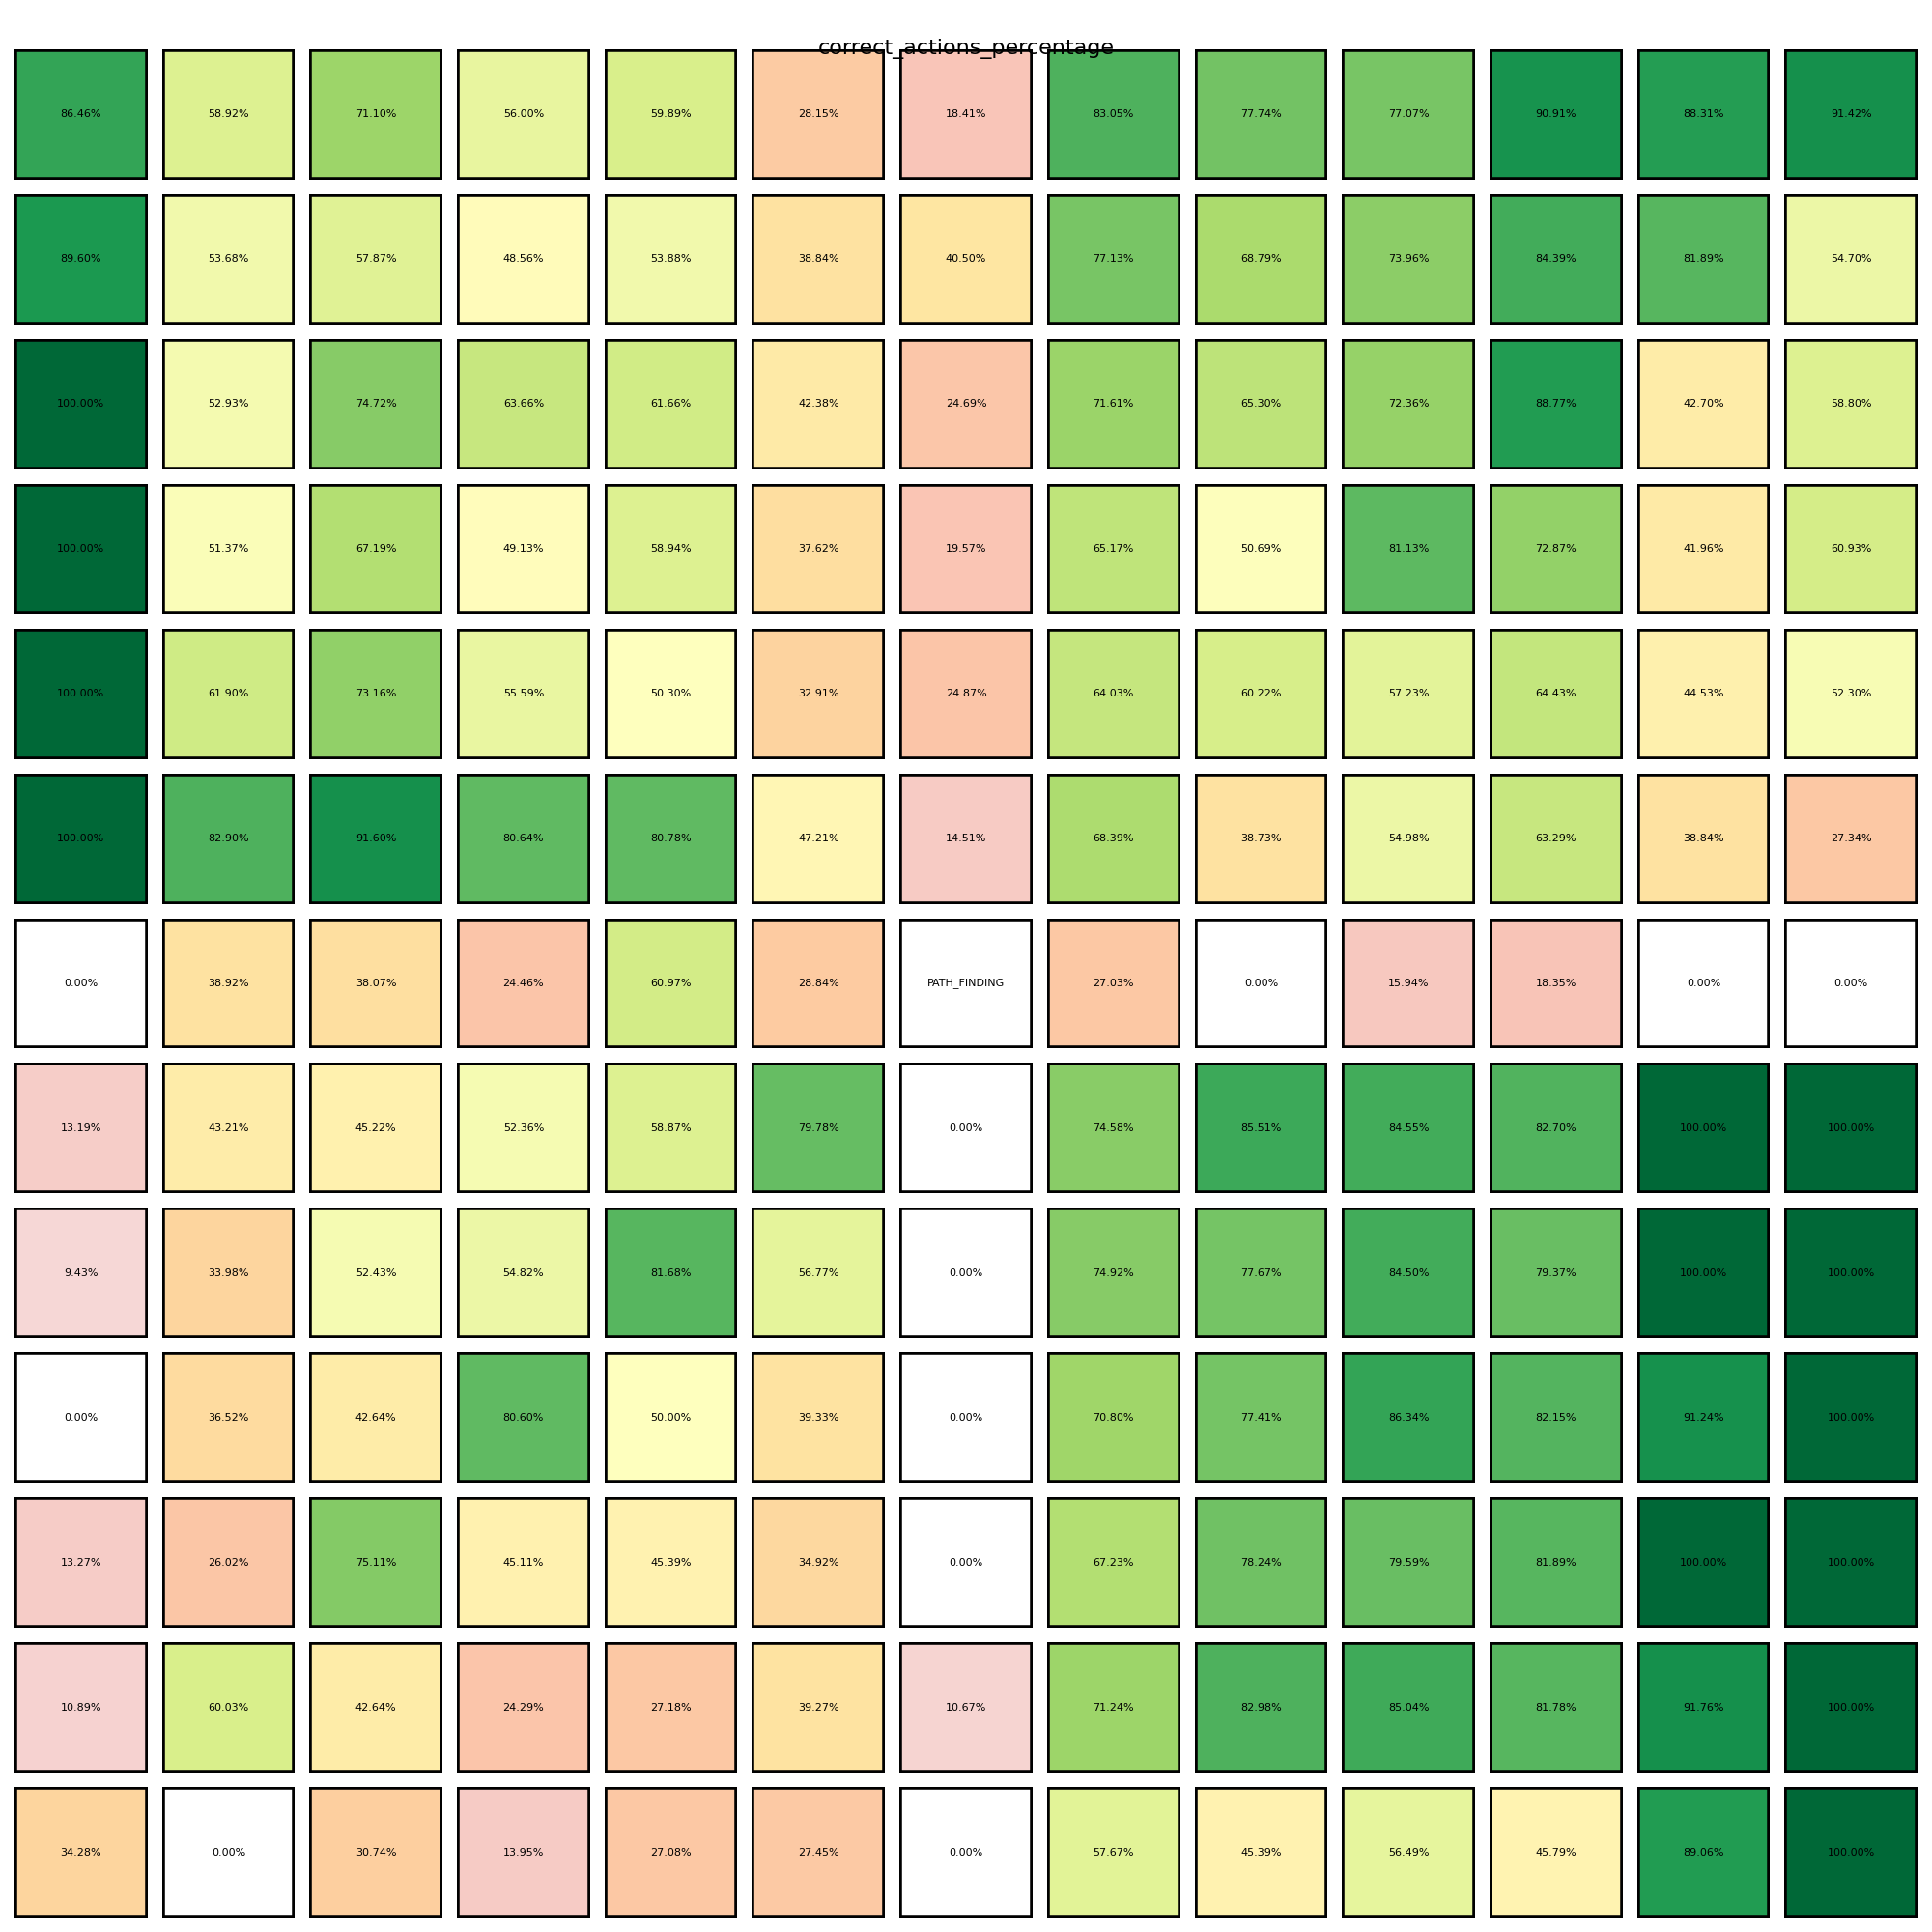
\includegraphics[width=\textwidth]{
      images/results_discussion/correctness_hm_BL.png
    }
    \caption{Bottom Left Orientation}
    \label{fig:heatmapBL}
  \end{minipage}
  \hfill
  \begin{minipage}[b]{0.45\textwidth}
    \centering
    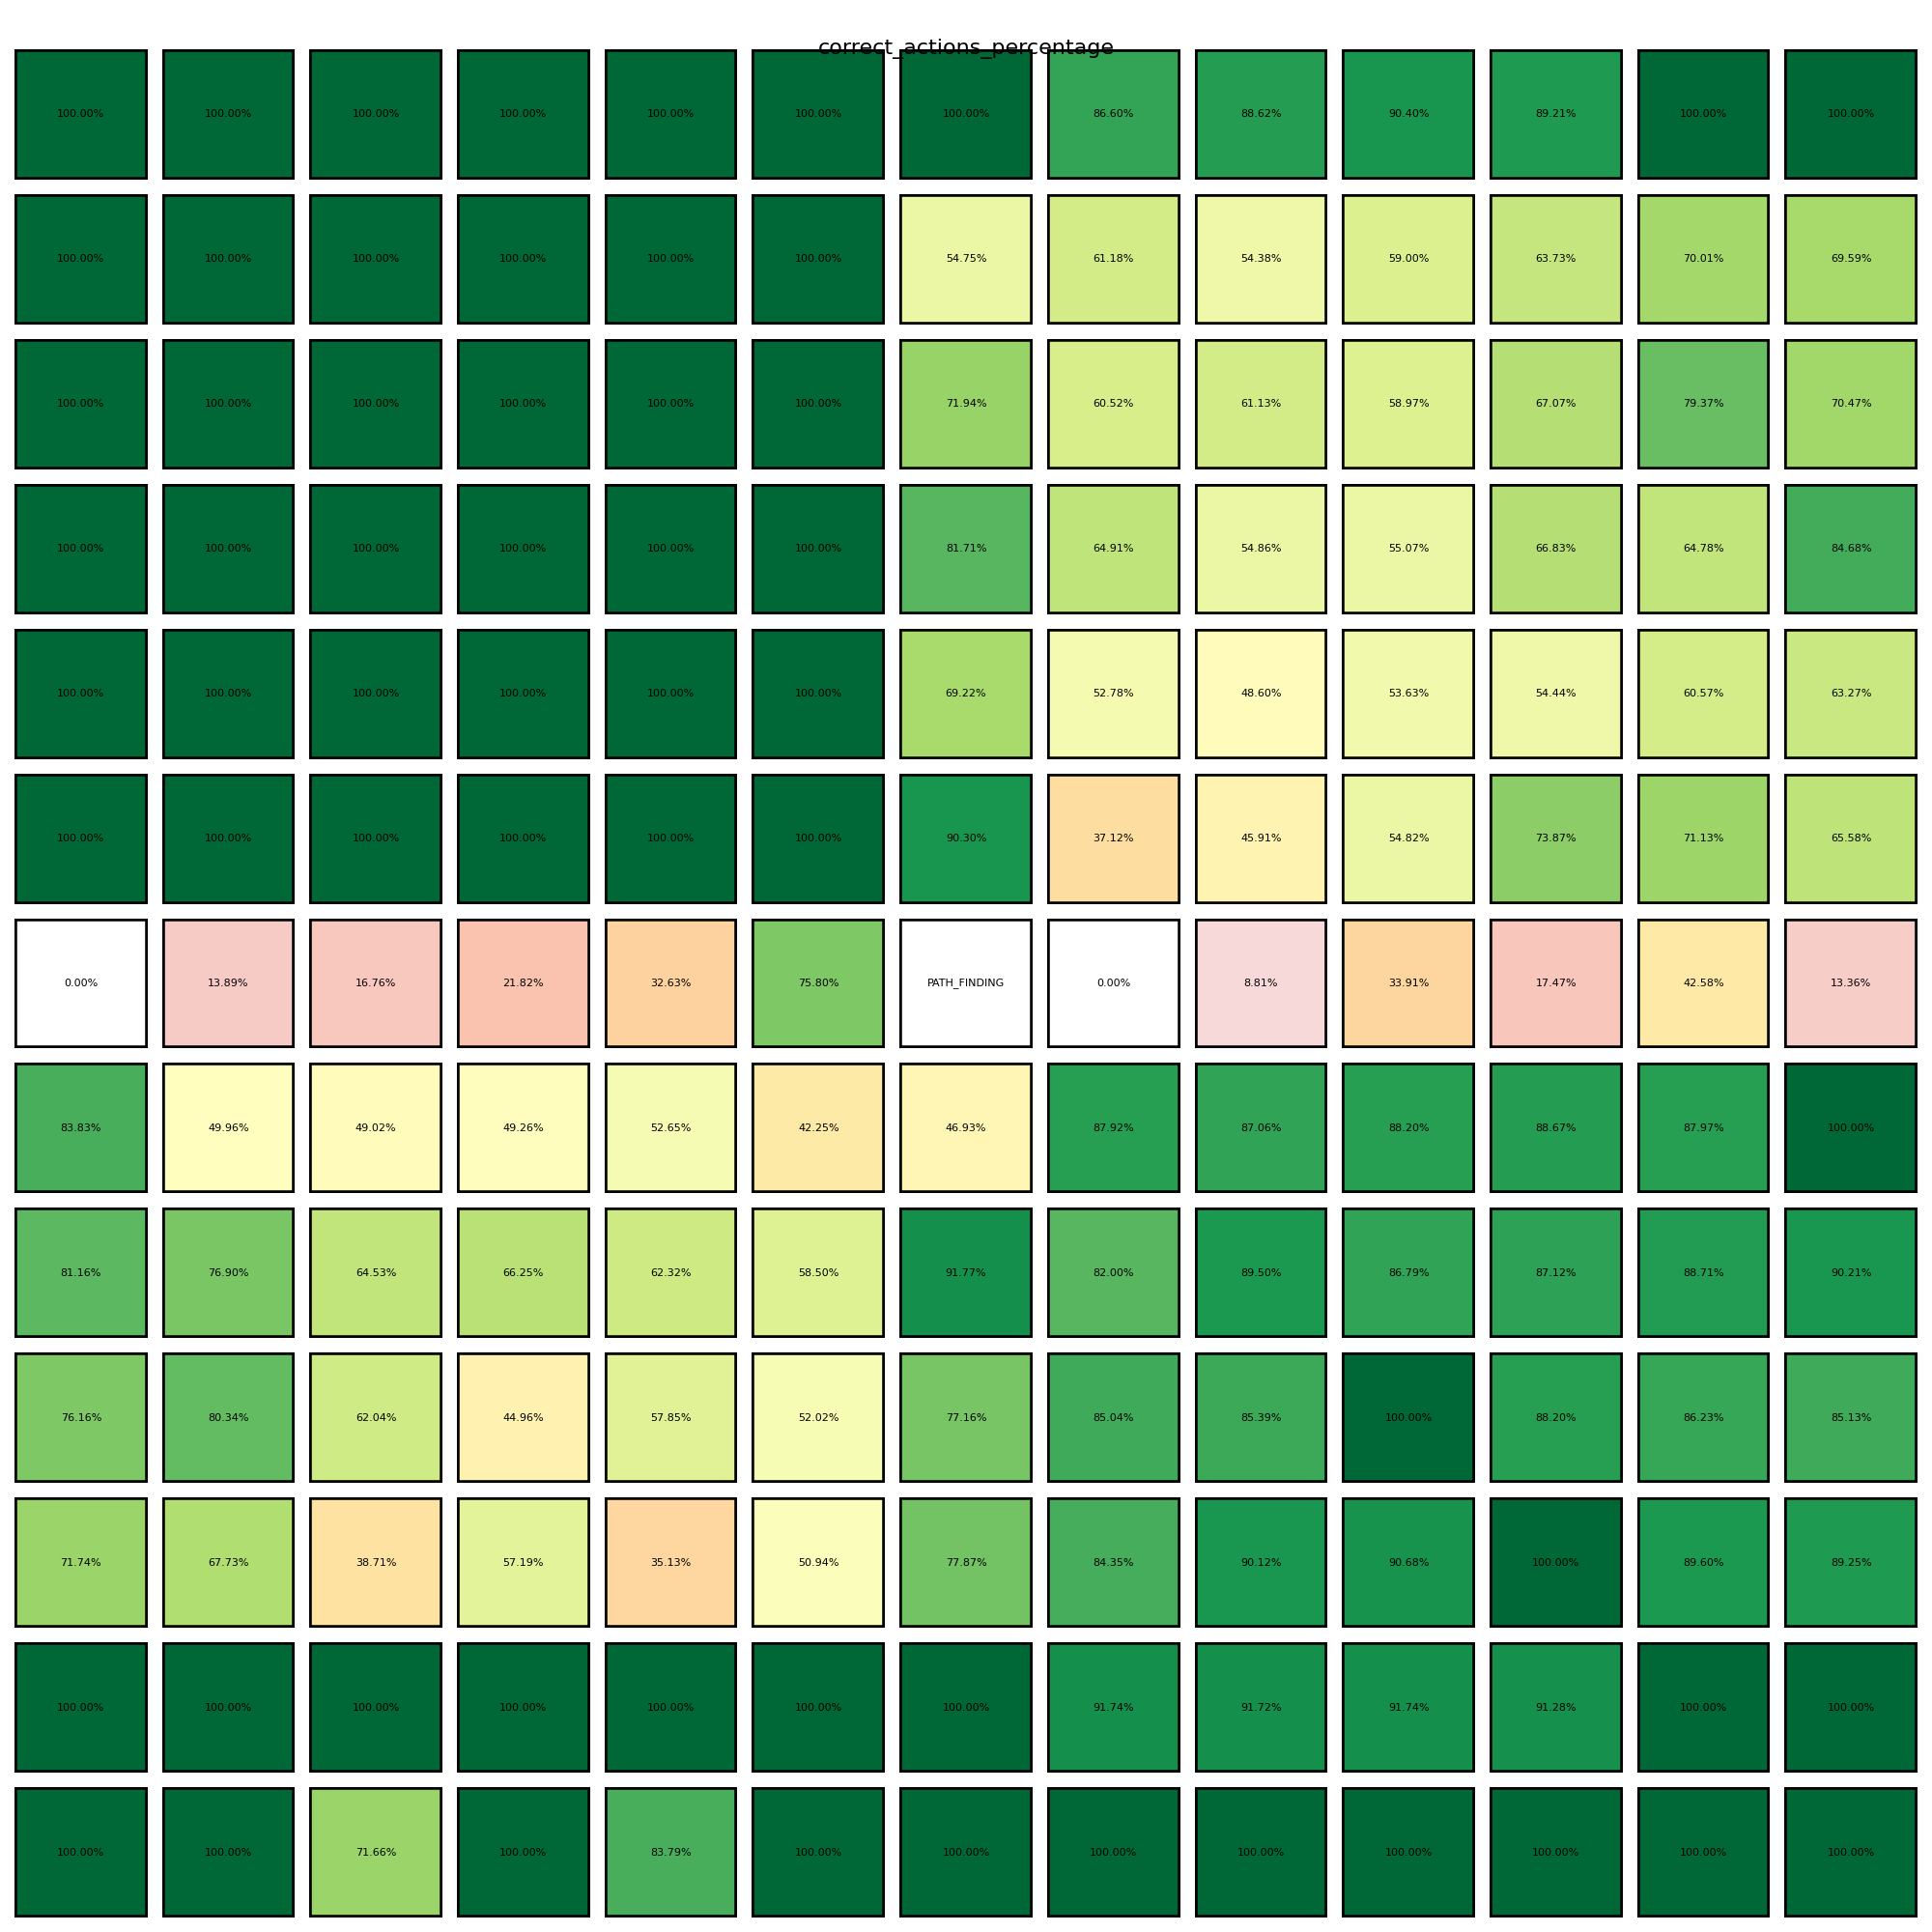
\includegraphics[width=\textwidth]{
      images/results_discussion/correctness_hm_TL.png
    }
    \caption{Top Left Orientation}
    \label{fig:heatmapTL}
  \end{minipage}
  \caption{Heatmaps showing correctness with different map orientations}
  \label{fig:orientation_correctness}
\end{figure}

\subsection{Comparison of Orientations}

When comparing the two orientations, we found that in the top-left origin
version, 154 tiles had one of the correct actions as the most probable choice.
In contrast, in the bottom-left origin version, only 104 tiles had a correct
action as the highest-probability choice. The comparison between the two orientations
reveals a clear preference for the top-left origin. The model performed
significantly better when using this orientation, as shown by the following accuracy
metrics:
\begin{itemize}
  \item Top-left origin: 92\% of the tiles had the correct action as the most probable
    one.

  \item Bottom-left origin: 62\% of the tiles had the correct action as the most
    probable one.

  \item Top 3 actions comparison: 99\% vs. 93\% of the tiles contained the correct
    action within the top three choices.
\end{itemize}

These results strongly suggest that the model is inherently biased toward the top-left
origin orientation. This finding highlights the potential influence of data
structure representations on LLM-based decision-making and suggests that models
trained on structured data formats may develop spatial preferences that impact
their performance in spatial reasoning tasks.

\section{Stateless}
\label{sec:stateless}

What stateless means with reference to Section \ref{sec:stateful_and_stateless_agents_chapAD}.

Cost of each call in terms of tokens and USDs.

\subsection{Heatmaps}

lines of the goal bad, probably because only one action correct

if overlapping the same portion, different values of the heatmap

goal action (T/S) in the cells near the goal

FIG 5x5 from 5.3

FIG 13x13 from 6.1

[FIG 21x21]

same portions of the map (eg top right portion) systematically lower score.

\section{Stateful}
\label{sec:stateful}

Works, but bigger the map, the worse the performance.

Also difficult to test in very big maps since token limit is reached after few calls.
See figure

Also tried by sending the map in the first call, then wait and send every 5 or
10 messages, but either no working or still so frequent that the limit was reached
fast.

\section{``Path Finding''}

tested to reduce the size of the problem, similarly to what was cited in Section
\ref{sec:closest_cell_to_the_goal}

same but without take and deliver as actions in the prompt, but similar result.

[fig with path finding and pickup]

[fig correctness with path finding and pickup]

\section{Stateless and Stateful Combined results}
\label{sec:stateless_and_stateful_combined_results}

stateful works best for “LLMs are few-shot learners” and the chat history with
action-effect\_in\_the\_map helps the LLM understand the map and the target; also,
as we see in the stateless, if the agent ends up in particular portions of the map,
it goes into a loop and never comes out from there. The areas problem areas,
although in percentage terms they do not change much with respect to map size, in
real numbers they are also substantial portions of the map (so if, for example,
in a 3x3 map we have one problem cell and in a 21x21 map we have 49, in percentage
terms they are the same number, but if in the first case the agent ends up in
the problem cell very easily gets out of it and gets to the goal, in the second case
the agent does not come out anymore)

\section{Closest Cell to the Goal Problems}
\label{sec:closest_cell_to_the_goal_problems} more than one cell could bring the
agent closer to the final goal. [add image similar \ref{fig:extra} but with goal
one tile to the right]

show prompt

\section{Models Comparison}
\label{sec:models_comparison}

Pickup 5x5 pickup (4,4) 3.5 vs 4o vs 4o-mini